% ----------------------------------------------------------
\section{Calibração das leituras de Ozônio}
% ----------------------------------------------------------

\begin{figure}[h!]
    \centering
    \caption{Desempenho dos modelos de regressão aplicados para inferir as leituras de concentração de \acrshort{o3} medidas pela estação de referência}
    \begin{subfigure}{0.9\textwidth}
        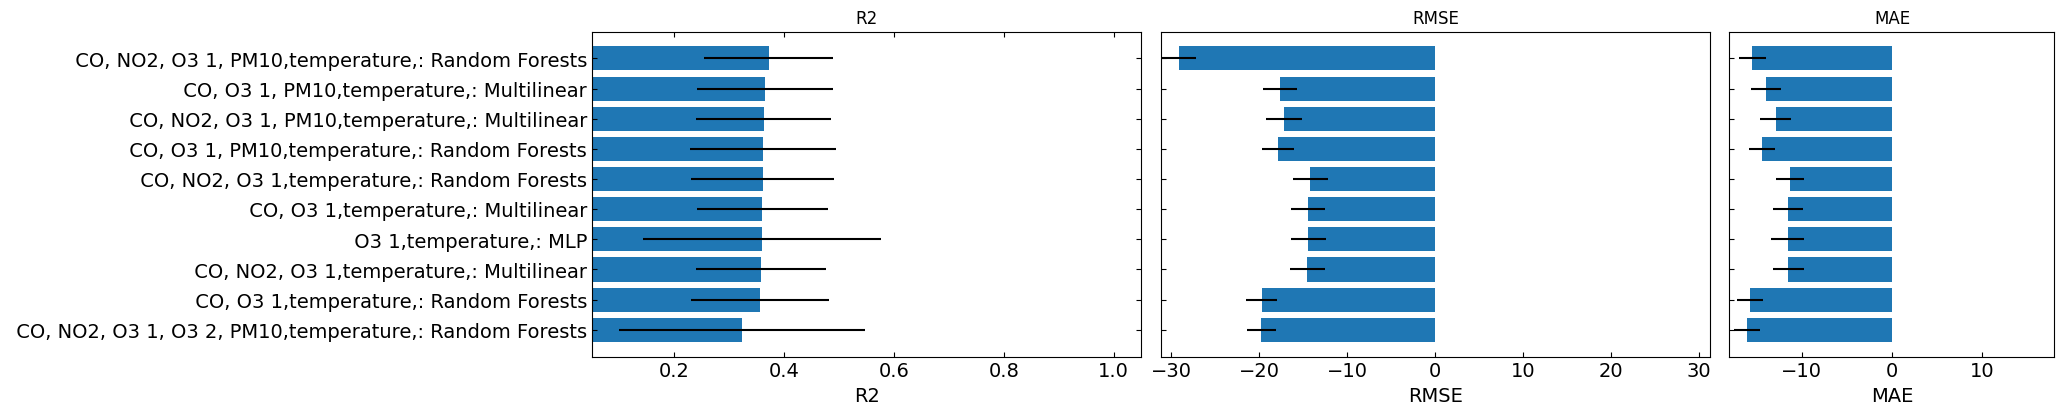
\includegraphics[width=\textwidth]{chapters/4-CALIBRAÇÃO MÚLTIPLOS SENSORES/Figuras/o3-all-models-performance.png}
        \caption{Valores de R2, RMSE e MAE obtidos pelos 10 modelos com maiores valores de R2}
        \label{fig:data-o3-all-models-performance}
    \end{subfigure}
    \begin{subfigure}{0.9\textwidth}
        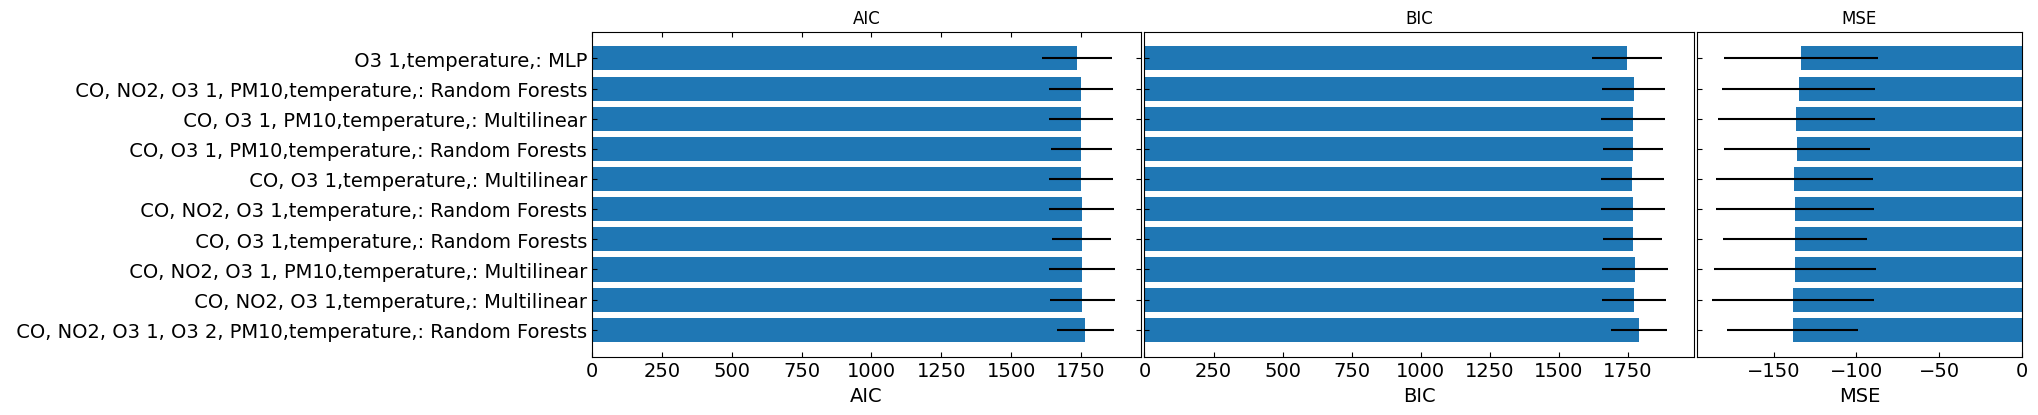
\includegraphics[width=\textwidth]{chapters/4-CALIBRAÇÃO MÚLTIPLOS SENSORES/Figuras/o3-all-models-complexity.png}
        \caption{Modelos com menores valores de \acrshort{aic} e \acrshort{bic}}
        \label{fig:data-o3-all-models-comlexity}
    \end{subfigure}
    \label{fig:data-o3-all-models-performance-comlexity}
\end{figure}

A Figura \ref{fig:data-o3-all-models-performance} apresenta os valores de R2 dos 10 melhores modelos de calibração calculados para as leituras de \acrshort{co}. Observa-se que os valores de R2 desses 10 modelos oscilaram entre 0.2 e 0.6, todos incluíram o \acrshort{co} e a temperatura. Apenas dois modelos não foram regressões lineares, ocupando as posições 5 e 6 com regressões por Florestas Aleatórias. As Florestas, embora não tenham produzido os maiores valores de R2 médio, apresentaram menores valores de erro e valores de R2 máximo mais altos em comparação com os quatro modelos lineares que os antecederam. Já em termos de complexidade, observa-se que apenas o modelo de regressão por Florestas Aleatórias que considerou como variáveis de entrada as leituras de \acrshort{co}, dos dois sensores de \acrshort{o3}, de \acrshort{mp10} e temperatura, conseguiu estar entre os 10 com menores valores de \acrshort{aic}. Os modelos lineares por sua parte produziram os menores coeficientes de complexidade.

\begin{figure}[h]
    \centering
    \caption{Gráfico de dispersão das leituras do múltiplos sensores e a estação de referência para medição de \acrshort{o3}}
    \begin{subfigure}{0.49\textwidth}
        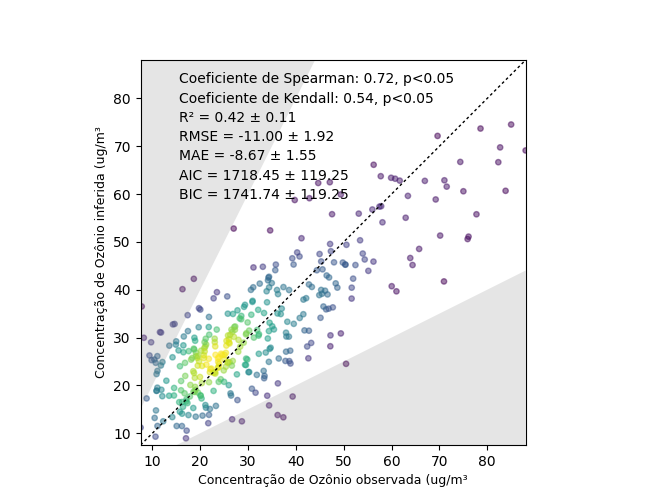
\includegraphics[width=\textwidth]{chapters/4-CALIBRAÇÃO MÚLTIPLOS SENSORES/Figuras/O3-co-no2-o31-pm10-T-Multilinear-Regression.png}
        \caption{Utilizando modelo de regressão linear multivariado com variáveis independentes: leituras de sensores CO-B4, NO2-B43F, OX-B431 (1), sensor de \acrshort{mp10} OPC-N3 e temperatura}
        \label{fig:data-co-no2-o31-pm10-T-reference-O3-corr-MLR}
    \end{subfigure}
    \hfill
    \begin{subfigure}{0.49\textwidth}
        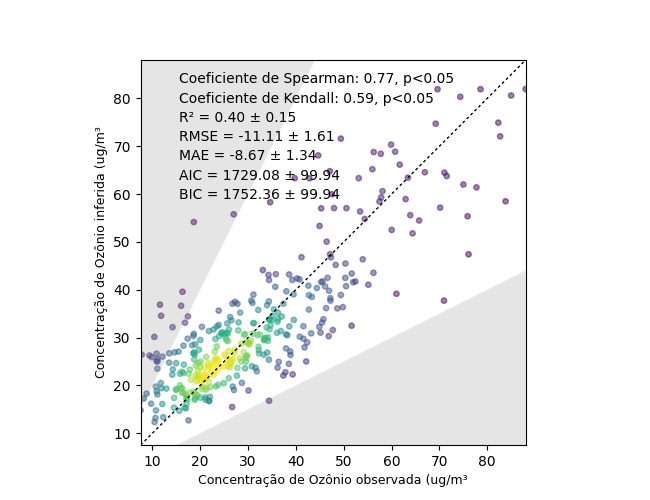
\includegraphics[width=\textwidth]{chapters/4-CALIBRAÇÃO MÚLTIPLOS SENSORES/Figuras/O3-co-o31-o32-pm10-T-RF-Regression.png}
        \caption{Utilizando modelo de regressão de Florestas Aleatórias com variáveis independentes: leituras de sensores CO-B4, OX-B431 (1 e 2), sensor de \acrshort{mp10} OPC-N3 e temperatura}
        \label{fig:data-co-o31-o32-pm10-T-reference-O3-corr-RF}
    \end{subfigure}
\end{figure}

As Figuras \ref{fig:data-co-no2-o31-pm10-T-reference-O3-corr-MLR} e \ref{fig:data-co-o31-o32-pm10-T-reference-O3-corr-RF} mostram os resultados de aplicar modelos de calibração baseados numa regressão linear multivariada e em Florestas Aleatórias respectivamente. O primeiro considera como variáveis independentes as leituras dos sensores CO-B4, NO2-B43F, OX-B431 (1), sensor de \acrshort{mp10} OPC-N3 e temperatura. Já o segundo considera como variáveis de entrada as leituras dos sensores CO-B4, OX-B431 (1 e 2), sensor de \acrshort{mp10} OPC-N3 e temperatura.